\documentclass{whutmod}
\usepackage[linesnumbered,ruled,lined]{algorithm2e}
\usepackage{amsmath,amsfonts,bm}
\usepackage{graphicx}
\usepackage{booktabs}
\usepackage{hyperref}
\usepackage{setspace}
\usepackage{natbib}
\bibliographystyle{unsrt}

% Team and member information
\team{10}
\membera{刘子川}
\joba{编程}
\memberb{程宇}
\jobb{建模}
\memberc{祁成}
\jobc{写作}

% Hyperlink setup
\hypersetup{
    colorlinks=true,
    linkcolor=black,
    citecolor=black
}

% Custom citation command for superscript
\newcommand{\upcite}[1]{\textsuperscript{\cite{#1}}}

% Title and problem number
\title{基于生命遗传算法与插板编码的充电路线规划}
\tihao{3}

% Set display style for math
\everymath{\displaystyle}

\begin{document}
    \maketitle
    \thispagestyle{empty}

    % Abstract
    \begin{abstract}
        影响无线传感器网络生命周期最重要的一个因素是能量,用移动充电器定期为传感器的电池补充能量至关重要。本文建立了基于变体TSP问题的优化模型,采用随机梯度下降、$LU$分解法以及插板编码嵌入的生命遗传算法对模型进行求解。

        针对问题一,对移动充电器(MC)的充电有效距离分类讨论,分别建立有线充电设备与无线充电设备的路线优化模型,并用生命遗传算法与随机梯度下降进行优化求解最佳充电路线。当设备为有线充电设备时,问题一即为经典TSP问题,使用生命遗传算法优化可得MC最短行驶路程为\textbf{11482.8m}。当设备为无线充电设备时,将随机梯度下降嵌入目标函数求解,分别可算当充电有效距离为\textbf{50m}和\textbf{100m}时的MC最短行驶路程为\textbf{11051.8m}和\textbf{9251.6m}。最后对实验结果进行灵敏度分析,分析充电有效距离与最短行驶路径间的关系。

        针对问题二,建立基于传输能量守恒的单MC能耗模型,并在固定周期遍历充电模型的基础上划分周期,从时间维度考察能量收支关系。在传感器电量满足阈值要求的极限情况下,将充电过程中的能量流动关系转化为与驻留期相关的矩阵方程。根据目标矩阵的代数特征,采用\bm{$LU$}分解法求解化简后的关于驻留期分布的线性方程组,最后由驻留期与电池容量关系确定电池阈值容量分布,结果如表~\ref{biao2}所示。对求解结果进行灵敏度分析,从实际角度考察MC充电半径等因素对传感器电池容量分布稳定性的影响。

        针对问题三,对于4辆MC同时执行充电任务的情况,在问题一模型的基础上设计插板式编码,优化求解该多旅行商问题。使用插板式编码重新构造决策变量,即对于4辆MC的整体路线,在决策序列中插入3块无意义挡板基因,使用生命遗传算法优化求解最短充电路线与其对应的电池容量分布。解得最短路程为\textbf{12950m},电池最小容量结果如表~\ref{adfs}所示。分析结果表明,增派MC不能降低路上的能量消耗,但能降低传感器网络对传感器电池容量的要求。

        本文的优点为:1. 结合无线能量传输技术的实际应用,在无线可充电传感器网络的固定周期遍历充电模型的基础上引入无线充电圆域半径,分别建立基于传输能量守恒的单MC和多MC能耗模型,拓广了模型应用范围。2. 从时间维度考察能量收支关系,利用$LU$分解法求解电池容量分布,具有无需判定矩阵是否正定,浮点数操作总量在$O(n^2)$等优点。3. 设计了生命遗传算法求解MC能耗模型中的最小能量消耗路线,有效防止算法陷入局部最优解,抑制算法早熟,兼顾了局部搜索与全局搜索能力。

        \keywords{
            生命遗传算法 \quad
            随机梯度下降 \quad
            \bm{$LU$}分解法 \quad
            插板式编码
        }
    \end{abstract}

    % Table of contents
    \thispagestyle{empty}
    \tableofcontents
    \setcounter{page}{0}
    \newpage

    % Problem restatement
    \section{问题重述}
        \subsection{问题背景}
            由部署在监控区域的大量低成本微传感器节点组成的网络系统,称为无线传感器网络(Wireless Sensor Network,WSN)。WSN节点通过无线信道相互通信,协同感知、收集和处理监控区域内传感对象的信息,然后将信息发送给观察者\upcite{1}。因此,WSN广泛应用于自然灾害预警、环境监测、战场监视等领域\upcite{2}。

            能源对无线传感器网络的发展至关重要。传感器节点通常由装载电池或超级电容器供电,但由于传感器节点尺寸较小,装载的电池容量有限,有时因为维护成本过高而无法延长无线传感器网络的生命周期,这限制了无线传感器网络的发展和应用。前人采用能量平衡\upcite{4,5}、移动传感器\upcite{6,7}和移动收集器等方案来节省能量,从而达到延长网络生命周期的目的。然而,这些方案仅降低能量消耗率,不能真正延长WSN的生命周期。

            在按需充电结构的无线可充电传感器网络(Wireless Rechargeable Sensor Network,WRSN)中,节点主动监视其自身的剩余能量,当其能量水平低于某个阈值时,向基站(BS)发送充电请求。BS根据某些充电规则对请求节点建立充电调度队列,并将该调度发送给无线充电设备(WCD),从而引导WCD为节点进行充电服务\upcite{3},如图~\ref{lasbel}所示。传统的调度方案只考虑时间、空间或两者混合因素。由于受到空间、时间和能量因素的制约,传统的调度方案仅能满足少量的充电请求节点,这导致WRSN在繁忙的网络环境中生命周期较短\upcite{3}。为了减小移动充电器在路上的能量消耗,需要合理规划移动充电器的充电路线。

            \begin{figure}[H]
                \centering
                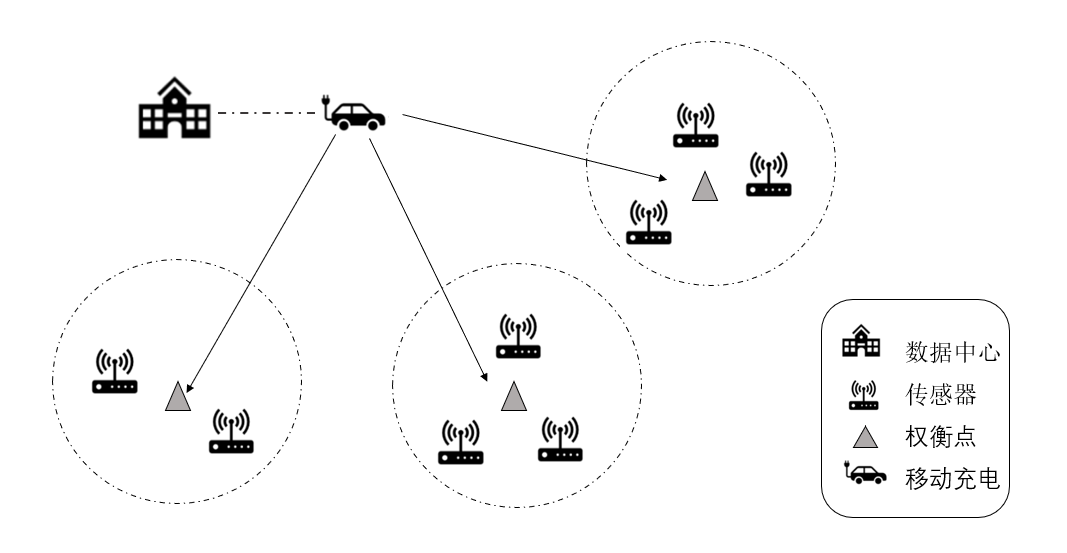
\includegraphics[width=\textwidth]{figures/demo.png}
                \caption{无线可充电传感器网络架构示意图}\label{lasbel}
            \end{figure}

        \subsection{问题概述}
            围绕相关附件和条件要求,研究一个或多个移动充电器在各传感器间的充电路线方案,依次提出以下问题:

            \textbf{问题一:} 当只派出一个移动充电器时,如何规划移动充电器的充电路线才能最小化移动充电器在路上的能量消耗?

            \textbf{问题二:} 在只派出一个移动充电器的情况下,若采用问题一中规划出来的充电路线,每个传感器的电池容量应至少是多大才能保证整个系统一直正常运行?

            \textbf{问题三:} 为了提高充电效率,同时派出4个移动充电器进行充电,在这种情况下应如何规划移动充电器的充电路线以最小化所有移动充电器在路上的总能量消耗?每个传感器的电池容量应至少是多大才能保证整个系统一直正常运行?

    % Model assumptions
    \section{模型假设}
        \begin{itemize}
            \item[(1)] 假设充电场景不属于时变充电方案,即传感器节点充电时单位时间的收发数据能量不随时间改变。
            \item[(2)] 考虑移动充电器(MC)可以同时为多个节点进行无线充电,即其具有一定的充电范围,并且在此范围内充电场的能级不随距离而发生变化。
            \item[(3)] 由于传感器分布区域较小,本文忽略地球曲率的影响,即假设所有传感器分布在同一个二维平面上。
            \item[(4)] 假设移动充电器在移动时的能量消耗功率为恒定值,即其不随移动路段和工作时间而改变。
        \end{itemize}

    % Symbol description
    \section{符号说明}
        \begin{table}[H]
            \centering
            \setlength{\tabcolsep}{12mm}
            \begin{tabular}{cc}
                \toprule[1.5pt]
                \multicolumn{1}{m{5cm}}{\centering 符号} & \multicolumn{1}{m{5cm}}{\centering 说明} \\
                \midrule[1pt]
                $L$ & 最低能耗对应的MC行驶总里程 \\
                $s_i$ & 第$i$个传感器 \\
                $r$ & 充电速率 \\
                $t_i$ & MC在第$i$个传感器处的驻留期 \\
                $f$ & 传感器正常工作的电量阈值 \\
                $R$ & 无线充电圆域半径 \\
                $v$ & MC行驶速率 \\
                $c_i$ & 第$i$个传感器电量消耗速率 \\
                $\alpha$ & 所有传感器间的距离中的最小值 \\
                \bottomrule[1.5pt]
            \end{tabular}
            \begin{tablenotes}
                \item 注:表中未说明的符号以首次出现处为准
            \end{tablenotes}
        \end{table}

    % Problem 1: Model establishment and solution
    \section{问题一模型的建立与求解}
        \subsection{问题描述与分析}
            问题一要求充电路线最小化移动充电器在路上的能量消耗。为使无线传感器网络(WSN)持续运行,移动充电器(MC)必须在每个生命周期中访问所有传感器节点并完成充电后返回数据中心。要使MC在路上的能量消耗最小,即每个周期内MC移动的路程最小。当MC为传统短程有线充电设备时,该问题可转化为经典TSP问题。

            随着无线充电技术的发展,WSN的充电任务由负载无线充电设备的移动充电器(WCV)完成。WCV可在距离目标传感器一定范围内执行无线充电,且可同时为多个传感器充电,假设在此范围内充电场的能级不随距离变化。本节优化求解不同充电有效距离下的最佳充电路线。

            本节首先假设MC为短程有线充电设备($R=0$),将问题转化为TSP优化模型,使用生命遗传算法求解。然后假设MC为无线充电设备,分为两种情况:当$0<R<\frac{\alpha}{2}$($\alpha$为传感器间最小距离),MC每次最多为一个传感器充电,使用随机梯度下降嵌入生命遗传算法优化;当$R \geqslant \frac{\alpha}{2}$,MC可同时为多个传感器充电,修改编码方式合并可充电区域重叠的传感器,求解最佳路径。问题一的思维流程图如图~\ref{asdf}所示。

            \begin{figure}[H]
                \centering
                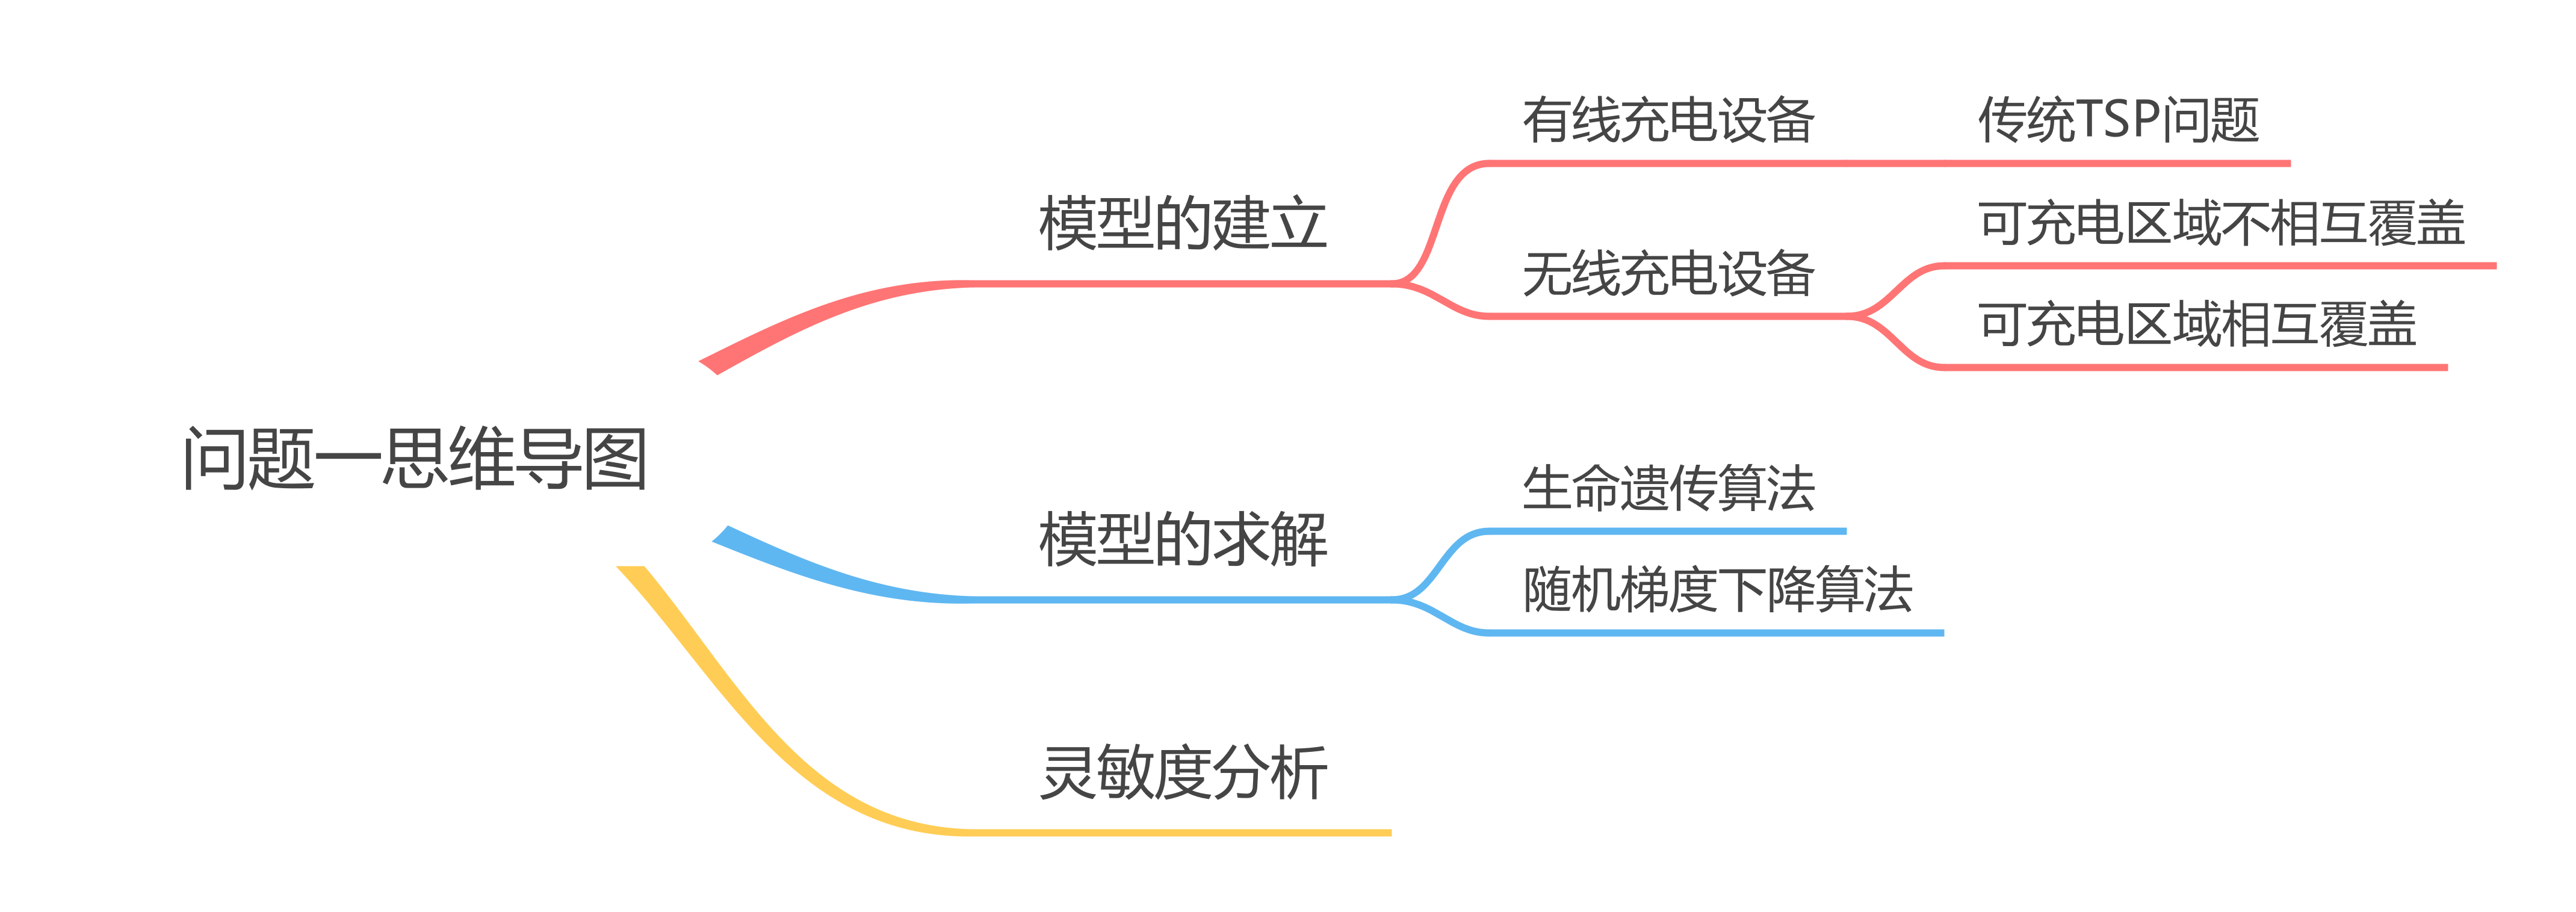
\includegraphics[width=\textwidth]{figures/1.png}
                \caption{问题一思维流程图}\label{asdf}
            \end{figure}

        \subsection{模型的建立}
            \subsubsection{有线充电设备模型}
                定义传感器坐标点集为$S=\{s_k \mid 1 \leqslant k \leqslant 29, k \in \mathbb{Z}\}$,其中$s_k$表示附件中第$k$号传感器的坐标。当MC为有线充电设备($R=0$),问题转化为TSP问题。假设MC移动时能量消耗功率为定值,为最小化能量消耗,需最小化每个周期的总路程。MC的充电路线表示为二维有限序列:
                \begin{gather}
                    P = [p_1, \dots, p_i, \dots, p_{29}],
                \end{gather}
                其中$p_i(x_i, y_i) \in S, (1 \leqslant i \leqslant 29, i \in \mathbb{Z})$表示MC经过的第$i$个传感器的坐标,且$\forall i \neq j, p_i \neq p_j$。任意两点$p_i(x_i, y_i)$和$p_j(x_j, y_j)$的欧式距离为:
                \begin{gather*}
                    d(p_i, p_j) = \sqrt{(x_i - x_j)^2 + (y_i - y_j)^2}.
                \end{gather*}
                以MC行驶路程为优化目标,目标函数为:
                \begin{gather*}
                    L(P_n) = d(p_0, p_1) + d(p_0, p_{29}) + \sum_{i=1}^{28} d(p_i, p_{i+1}),
                \end{gather*}
                其中$p_0(x_0, y_0)$为数据中心坐标,$L(P_n)$为路线$P_n$的总路程。优化模型为:
                \begin{gather}
                    \min L(P_n), \\
                    s.t. \left\{
                    \begin{matrix}
                        p_i(x_i, y_i) \in S, (1 \leqslant i \leqslant 29, i \in \mathbb{Z}), \\
                        \forall i \neq j, p_i \neq p_j.
                    \end{matrix}
                    \right.
                \end{gather}

            \subsubsection{无线充电设备模型}
                当MC为无线充电设备,充电有效距离为$R$,假设在有效距离内充电场能级不随距离变化,即当MC位置$p_m(x_m, y_m)$与传感器$s_i(x_{si}, y_{si})$满足$d(p_m, s_i) \leqslant R$时,充电速率为$r$(mA/s)。当:
                \begin{gather}
                    0 < R < \frac{1}{2} \min_{1 \leqslant i, j \leqslant 29, i \neq j} \{ d(s_i, s_j) \},
                \end{gather}
                MC每次最多为一个传感器充电,充电路线如图~\ref{asffa}所示。

                \begin{figure}[H]
                    \centering
                    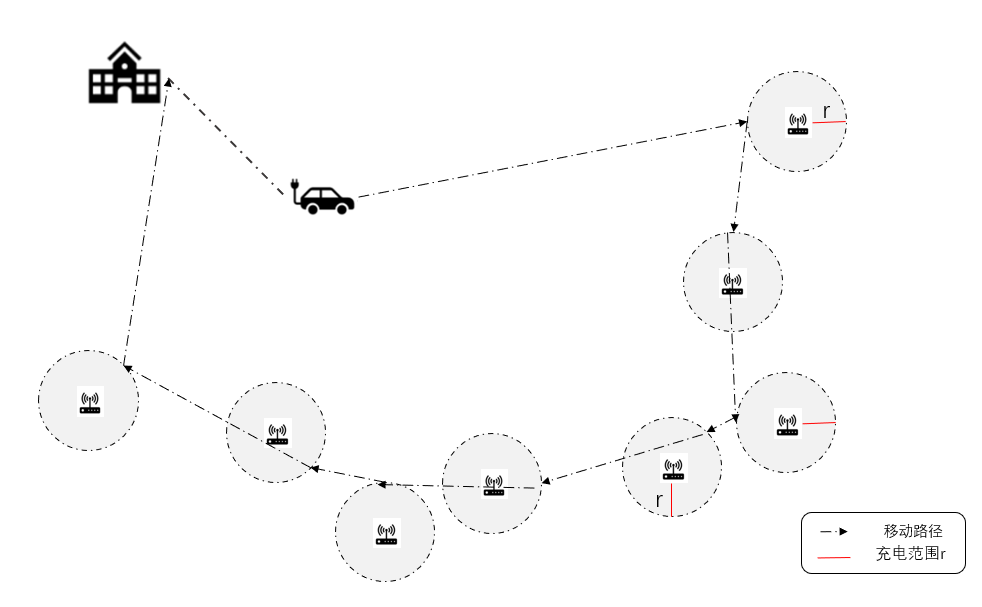
\includegraphics[width=.8\textwidth]{figures/bufu.png}
                    \caption{充电区域不重叠时充电路线示意图}\label{asffa}
                \end{figure}

                充电路线仍为:
                \begin{gather}
                    P = [p_1, \dots, p_i, \dots, p_{29}],
                \end{gather}
                其中$p_i(x_i, y_i)$为MC停留点坐标,满足充电距离约束:
                \begin{gather}
                    \forall i \in [1, 29]: \min_{p_j \in P} \{ d(s_i, p_j) \} \leqslant R,
                \end{gather}
                且每个停留点最多为一个传感器充电,不同停留点充电目标不同:
                \begin{gather}
                    \forall i, j \in [1, 29], i \neq j: \arg\min_{s \in S} \{ d(p_i, s) \} \neq \arg\min_{s \in S} \{ d(p_j, s) \},
                \end{gather}
                所有传感器均被充电:
                \begin{gather}
                    \bigcup_{i=1}^{29} \arg\min_{s \in S} \{ d(p_i, s) \} = S.
                \end{gather}
                目标函数为:
                \begin{gather*}
                    L(P) = d(p_0, p_1) + d(p_0, p_{29}) + \sum_{i=1}^{28} d(p_i, p_{i+1}),
                \end{gather*}
                优化模型为:
                \begin{gather}
                    \min L(P), \\
                    s.t. \left\{
                    \begin{matrix}
                        1 \leqslant i \leqslant 29, i \in \mathbb{Z}, \\
                        0 < R < \frac{1}{2} \min_{1 \leqslant i, j \leqslant 29, i \neq j} \{ d(s_i, s_j) \}, \\
                        \forall i \in [1, 29]: \min_{p_j \in P} \{ d(s_i, p_j) \} \leqslant R, \\
                        \bigcup_{i=1}^{29} \arg\min_{s \in S} \{ d(p_i, s) \} = S, \\
                        \forall i, j \in [1, 29], i \neq j: \arg\min_{s \in S} \{ d(p_i, s) \} \neq \arg\min_{s \in S} \{ d(p_j, s) \}.
                    \end{matrix}
                    \right.
                \end{gather}

                当$R \geqslant \frac{\alpha}{2}$,多个传感器可充电区域重叠,如图~\ref{ngf}所示。

                \begin{figure}[H]
                    \centering
                    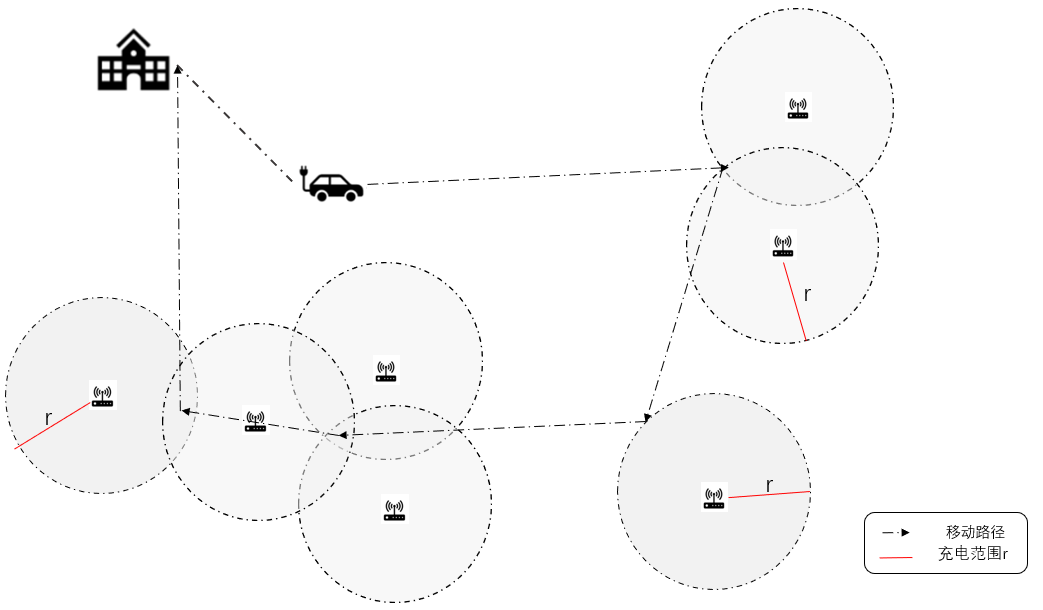
\includegraphics[width=.8\textwidth]{figures/fugai.png}
                    \caption{充电区域重叠时充电路线示意图}\label{ngf}
                \end{figure}

                若$k$个传感器可充电区域重叠,停留点数量为$30-k$,充电路线为:
                \begin{gather}
                    P_k = [p_1, \dots, p_i, \dots, p_{30-k}],
                \end{gather}
                目标函数为:
                \begin{gather}
                    L(P_k) = d(p_0, p_1) + d(p_0, p_{30-k}) + \sum_{i=1}^{29-k} d(p_i, p_{i+1}),
                \end{gather}
                每个传感器可充电范围内至少有一个停留点:
                \begin{gather}
                    \forall s_i \in S: \min_{p_j \in P_k} \{ d(s_i, p_j) \} \leqslant R.
                \end{gather}
                优化模型为:
                \begin{gather}
                    \min L(P_k), \\
                    s.t. \left\{
                    \begin{matrix}
                        1 \leqslant i \leqslant 29, i \in \mathbb{Z}, \\
                        R \geqslant \frac{1}{2} \min_{1 \leqslant i, j \leqslant 29, i \neq j} \{ d(s_i, s_j) \}, \\
                        \forall s_i \in S: \min_{p_j \in P_k} \{ d(s_i, p_j) \} \leqslant R.
                    \end{matrix}
                    \right.
                \end{gather}

        \subsection{模型的求解}
            本文针对$R=0$、$0<R<\frac{\alpha}{2}$和$R \geqslant \frac{\alpha}{2}$三种情况进行优化求解。$R=0$时为TSP问题,使用生命遗传算法(LGA)。$0<R<\frac{\alpha}{2}$时,将随机梯度下降(SGD)嵌入LGA适应度求解。$R \geqslant \frac{\alpha}{2}$时,合并重叠区域编码后使用内嵌SGD的LGA优化。

            \subsubsection{生命遗传算法}
                LGA在遗传算法基础上加入生命值衰减和个体死亡,防止陷入局部最优并抑制早熟。每个编码个体包括决策变量、适应度和剩余生命值,如图~\ref{saf}所示。

                \begin{figure}[H]
                    \centering
                    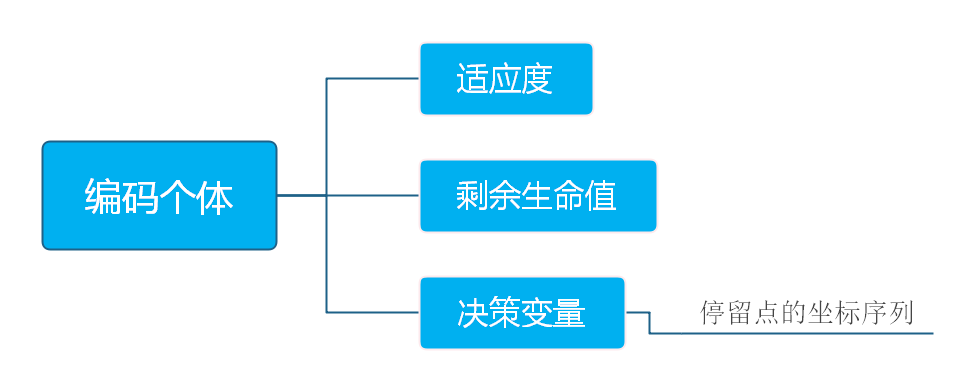
\includegraphics[width=.8\textwidth]{figures/lga.png}
                    \caption{生命遗传算法编码个体组成}\label{saf}
                \end{figure}

                \paragraph{初始化编码}
                    对遍历路径$P$进行整数编码:
                    \begin{gather*}
                        A_n = [a_{n1}, a_{n2}, \dots, a_{ni}, \dots, a_{n29}], \\
                        1 \leqslant a_i \leqslant 29, i \in \mathbb{Z}; \forall i \neq j: p_i \neq p_j,
                    \end{gather*}
                    其中$A_n$为解序列$P_n$的编码,$a_{ni}$表示第$i$次访问的传感器编号。随机生成初始解集$\{A_n\}_0$,$n=1,2,\dots,w$,$w$为种群容量。

                \paragraph{交叉}
                    在解集$\{A_n\}$中按随机顺序配对,采用顺序交叉生成子代。交叉操作如图~\ref{gbf}所示。

                    \begin{figure}[H]
                        \centering
                        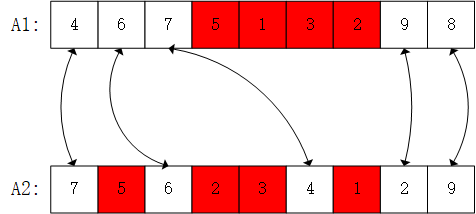
\includegraphics[width=.75\textwidth]{figures/cross.png}
                        \caption{顺序交叉}\label{gbf}
                    \end{figure}

                    选择$A_1$中一段编码作为保留基因,交换$A_1$和$A_2$的非保留基因,生成子代$H_1$和$H_2$。采用混合分组,父代均匀混合后,奇数编号个体与其相邻偶数编号个体交叉,生成子代集合$\{H_n\}$.

                \paragraph{变异}
                    采用改良圈算法变异,在染色体$A$中随机选取$a_i$和$a_j$($1 \leqslant i < j \leqslant 29$),颠倒$a_i$到$a_j$的顺序:
                    \begin{gather}
                        M = [a_1, \dots, a_i, a_{j-1}, a_{j-2}, \dots, a_{i+1}, a_j, \dots, a_{29}].
                    \end{gather}
                    每个染色体$A_n$以变异概率$\gamma$执行变异,生成子代集合$\{M_n\}$.

                \paragraph{赌轮选择}
                    将第$g$代染色体及其交叉、变异子代合并为解集$G_g = \{A, H, M\}$。$G_g$中第$i$个解$G_g(i)$被选入下一代的概率为:
                    \begin{gather}
                        P(G_g(i)) = \frac{f(G_g(i))}{\sum_{j=1}^{k} f(G_g(j))},
                    \end{gather}
                    其中$f(G_g(i))$为目标函数值(适应度)。在$G_g$中选择$w$次,生成下一代$\{A_n\}_{g+1}$.

                \paragraph{生命衰减}
                    每个染色体$\{A_n\}_{g+1}$生成时,初始生命值为正整数$H$:
                    \begin{gather}
                        Hp(A_n) = H.
                    \end{gather}
                    按适应度$f(A_n)$升序排列,前$p$个为优质个体,不衰减生命值。后$w-p$个个体生命值减1:
                    \begin{gather}
                        Hp(A_n) = Hp(A_n) - 1, \quad n = p, p+1, \dots, w.
                    \end{gather}
                    当$Hp(A_n) = 0$,剔除$A_n$,随机生成新解替代。伪代码如下:

                    \begin{algorithm}[H]
                        \caption{生命遗传算法}
                        \setstretch{0.7}
                        \LinesNumbered
                        \KwIn{种群规模: $w$; 迭代次数: $T$; 变异概率: $\gamma$; 初始生命值: $h$; 优质个体数量: $p$}
                        \KwOut{最优解: $X_{min}$}
                        \textbf{Initialize} $g \leftarrow 0$ \\
                        $\triangleright$ (初始化) \\
                        \For{$k = 1$ to $w$}{
                            $X_k = \text{randperm}(29)$ \\
                            $Hp(X_k) = h$
                        }
                        \While{$g \leqslant T$}{
                            $\triangleright$ (交叉) \\
                            \For{$k = 1$ to $w-1$ by 2}{
                                $\{H_k(g), H_{k+1}(g)\} = \text{Crossover}(X_k(g), X_{k+1}(g))$ \\
                                $Hp(H_k(g)) = h$; $Hp(H_{k+1}(g)) = h$
                            }
                            $\triangleright$ (变异) \\
                            \For{$k = 1$ to $w$}{
                                \If{$\text{rand}(0,1) < \gamma$}{
                                    $M_k(g) = \text{Mutation}(X_k(g))$ \\
                                    $Hp(M_k(g)) = h$
                                }
                            }
                            $\{S_k(g)\} \leftarrow \{H_k(g)\} + \{M_k(g)\} + \{X_k(g-1)\}$ \\
                            $\triangleright$ (赌轮选择) \\
                            \For{$k = 1$ to $w$}{
                                $X_k(g+1) = \text{Roulette}(\{S_k(g)\})$
                            }
                            $\text{sort}(\{X_k(g+1)\}, f(X_k(g+1)))$ \\
                            $\triangleright$ (生命衰减) \\
                            \For{$k = p+1$ to $w$}{
                                $Hp(X_k(g)) = Hp(X_k(g)) - 1$ \\
                                \If{$Hp(X_k(g)) = 0$}{
                                    $X_k(g) = \text{randperm}(29)$
                                }
                            }
                            $g \leftarrow g + 1$
                        }
                        \Return{$\arg\min \{f(X_k(g))\}$}
                    \end{algorithm}

            \subsubsection{随机梯度下降}
                当$R > 0$,采用随机梯度下降(SGD)优化目标函数$L(P_k)$,使用单个样本损失近似平均损失:
                \begin{gather}
                    \begin{matrix}
                        L(P, \Theta) = d(p_0, p_1, \theta_0) + d(p_0, p_{30-k}, \theta_{30}) + \sum_{i=1}^{30-k} d(p_i, p_{i+1}, \theta_i), \\
                        \nabla L(P, \Theta) = \frac{1}{m} \sum_{j=1}^{m} \nabla L(p_k, \theta_i),
                    \end{matrix}
                \end{gather}
                其中$P$为中心位置向量,$\Theta$为圆周角度参数,$d(p_i, p_{i+1})$为点间距离。参数更新公式为:
                \begin{gather}
                    \theta_{t+1} = \theta_t - \eta \nabla L(\theta_t),
                \end{gather}
                其中$\eta$为学习率。伪代码如下:

                \begin{algorithm}[H]
                    \caption{随机梯度下降}
                    \setstretch{1}
                    \LinesNumbered
                    \KwIn{中心位置: $P$; 角度: $\Theta$; 学习率: $\eta$}
                    \KwOut{更新后$\Theta$}
                    \textbf{Initialize} $\Theta \leftarrow 0$ \\
                    \For{$k = 1$ to $\text{max}$}{
                        $\theta_i \leftarrow \Theta[i]$ \\
                        $\nabla L(P, \Theta) = \frac{1}{m} \sum_{j=1}^{m} \nabla L(p_k, \theta_i)$ \\
                        \If{$\|\Theta\|^2 \leq \text{precision}$}{\textbf{break}}
                        $\theta_{t+1} = \theta_t - \eta \nabla L(\theta_t)$
                    }
                    \Return{$\Theta$}
                \end{algorithm}

                将优化后的$\Theta$代入$L(P_k, \Theta)$,计算最短距离,作为适应度继续执行LGA。

        \subsection{实验结果及分析}
            对于有线充电设备($R=0$),最短路径如图~\ref{sssssssssss}所示:

            \begin{figure}[H]
                \centering
                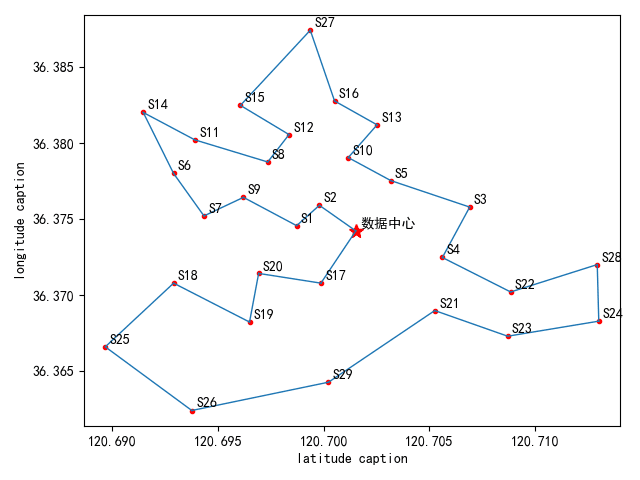
\includegraphics[width=.6\textwidth]{figures/w1.png}
                \caption{充电半径$R=0$时移动规划路径}\label{sssssssssss}
            \end{figure}

            规划路线为$[0, 2, 1, 9, 7, 6, 14, 11, 8, 12, 15, 27, 16, 13, 10, 5, 3, 4, 22, 28, 24, 23, 21, 29, 26, 25, 18, 19, 20, 17, 0]$,总距离为$11482.80289m$。

            对于无线充电设备,临界条件为$R=88.53m$。当$0<R<88.53m$,MC最多为一个传感器充电;当$R>88.53m$,可为多个传感器充电。路径如图~\ref{ssw}所示:

            \begin{figure}[H]
                \centering
                \subfigure[充电半径$0<R<88.53m$时移动规划路径]{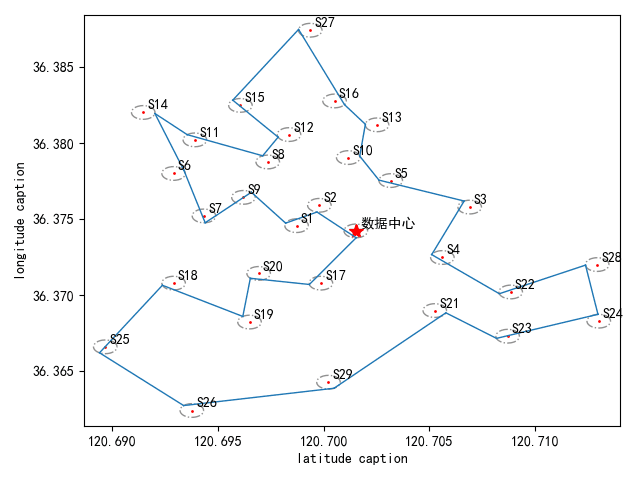
\includegraphics[height=6.5cm,width=7.5cm]{w2.png}}
                \subfigure[充电半径$R>88.53m$时移动规划路径]{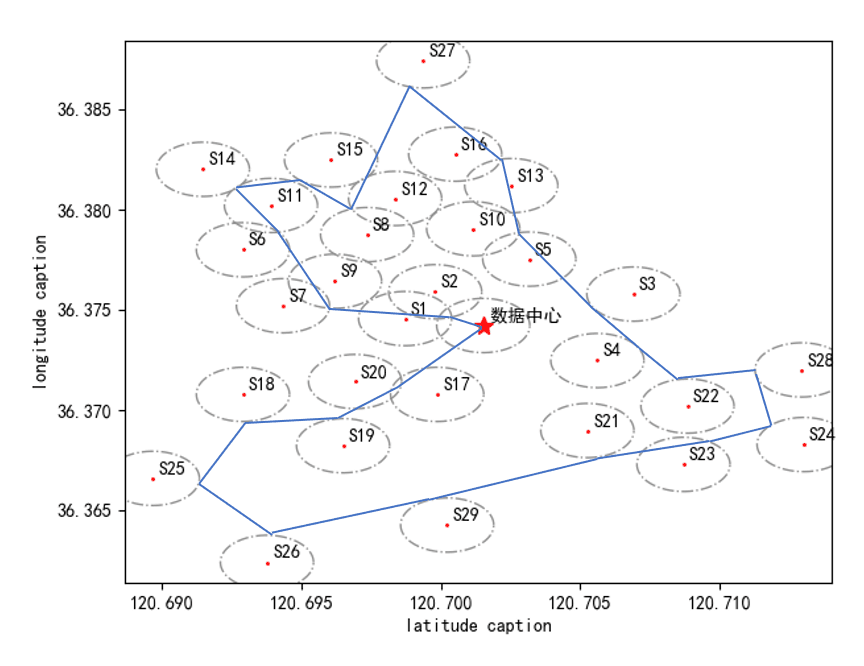
\includegraphics[height=6.5cm,width=7.5cm]{w3.png}}
                \caption{无线充电设备移动规划路径}\label{ssw}
            \end{figure}

            取$R=50m$,总距离为$11051.7684m$,路线为$[0, 2, 1, 9, 7, 6, 14, 11, 8, 12, 15, 27, 16, 13, 10, 5, 3, 4, 22, 28, 24, 23, 21, 29, 26, 25, 18, 19, 20, 17]$;取$R=100m$,总距离为$9251.6418m$。LGA收敛图如下:

            \begin{figure}[H]
                \centering
                \subfigure[充电半径$0 \leq R < 88.53m$时算法收敛图]{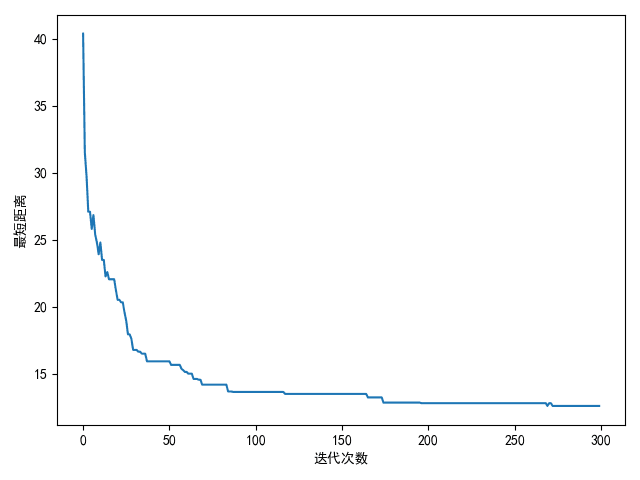
\includegraphics[height=6.5cm,width=7.5cm]{w11.png}}
                \subfigure[充电半径$R > 88.53m$时算法收敛图]{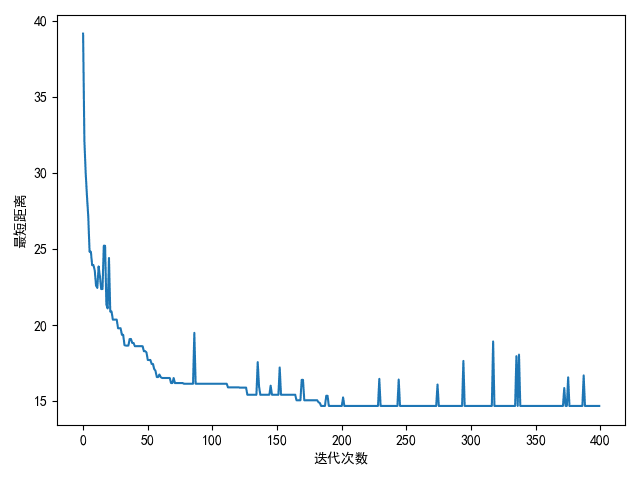
\includegraphics[height=6.5cm,width=7.5cm]{w22.png}}
                \caption{生命遗传算法收敛图}
            \end{figure}

            算法收敛速度快,复杂度低于遍历求解。小$R$时早熟问题解决较好,全局搜索能力强;大$R$时SGD引入振荡,但仍能找到局部最优解。

        \subsection{灵敏度分析}
            充电有效距离$R$影响总路程$L$。在$0m$至$80m$范围内变化,$L$的变化如图~\ref{ssssssssssssss}所示:

            \begin{figure}[H]
                \centering
                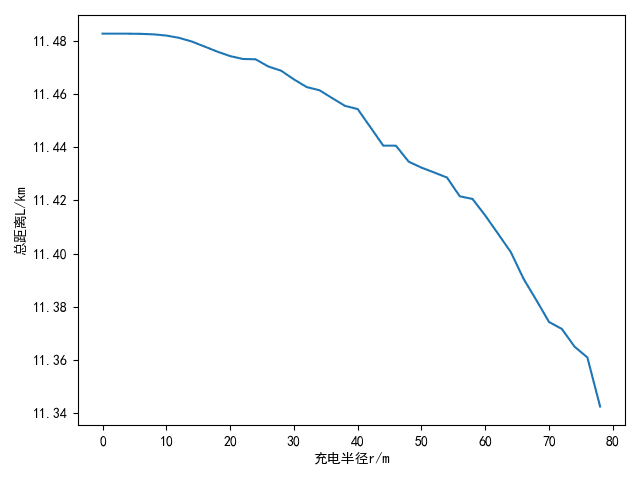
\includegraphics[width=.8\textwidth]{figures/ssss.png}
                \caption{充电半径$R$与总路程$L$关系}\label{ssssssssssssss}
            \end{figure}

            随$R$增加,$L$总体下降,符合实际。$L$下降不平滑,表明算法未完全找到全局最优解,但结果接近最优曲线。

    % Problem 2: Model establishment and solution
    \section{问题二模型的建立与求解}
        \subsection{问题描述与分析}
            问题二要求在问题一最优路线基础上,确定传感器最小电池容量分布。在固定周期$T$的遍历充电模型中,能量得失与时间成正比。本节将周期划分为驻留期和移动期。移动期和驻留期以恒定速率耗电,仅在驻留期充电。极限情况下,能量供需平衡对应最小容量。建立能量流动方程组,求解驻留时间分布,推导电池容量。思维流程图如图~\ref{ssssct}所示:

            \begin{figure}[H]
                \centering
                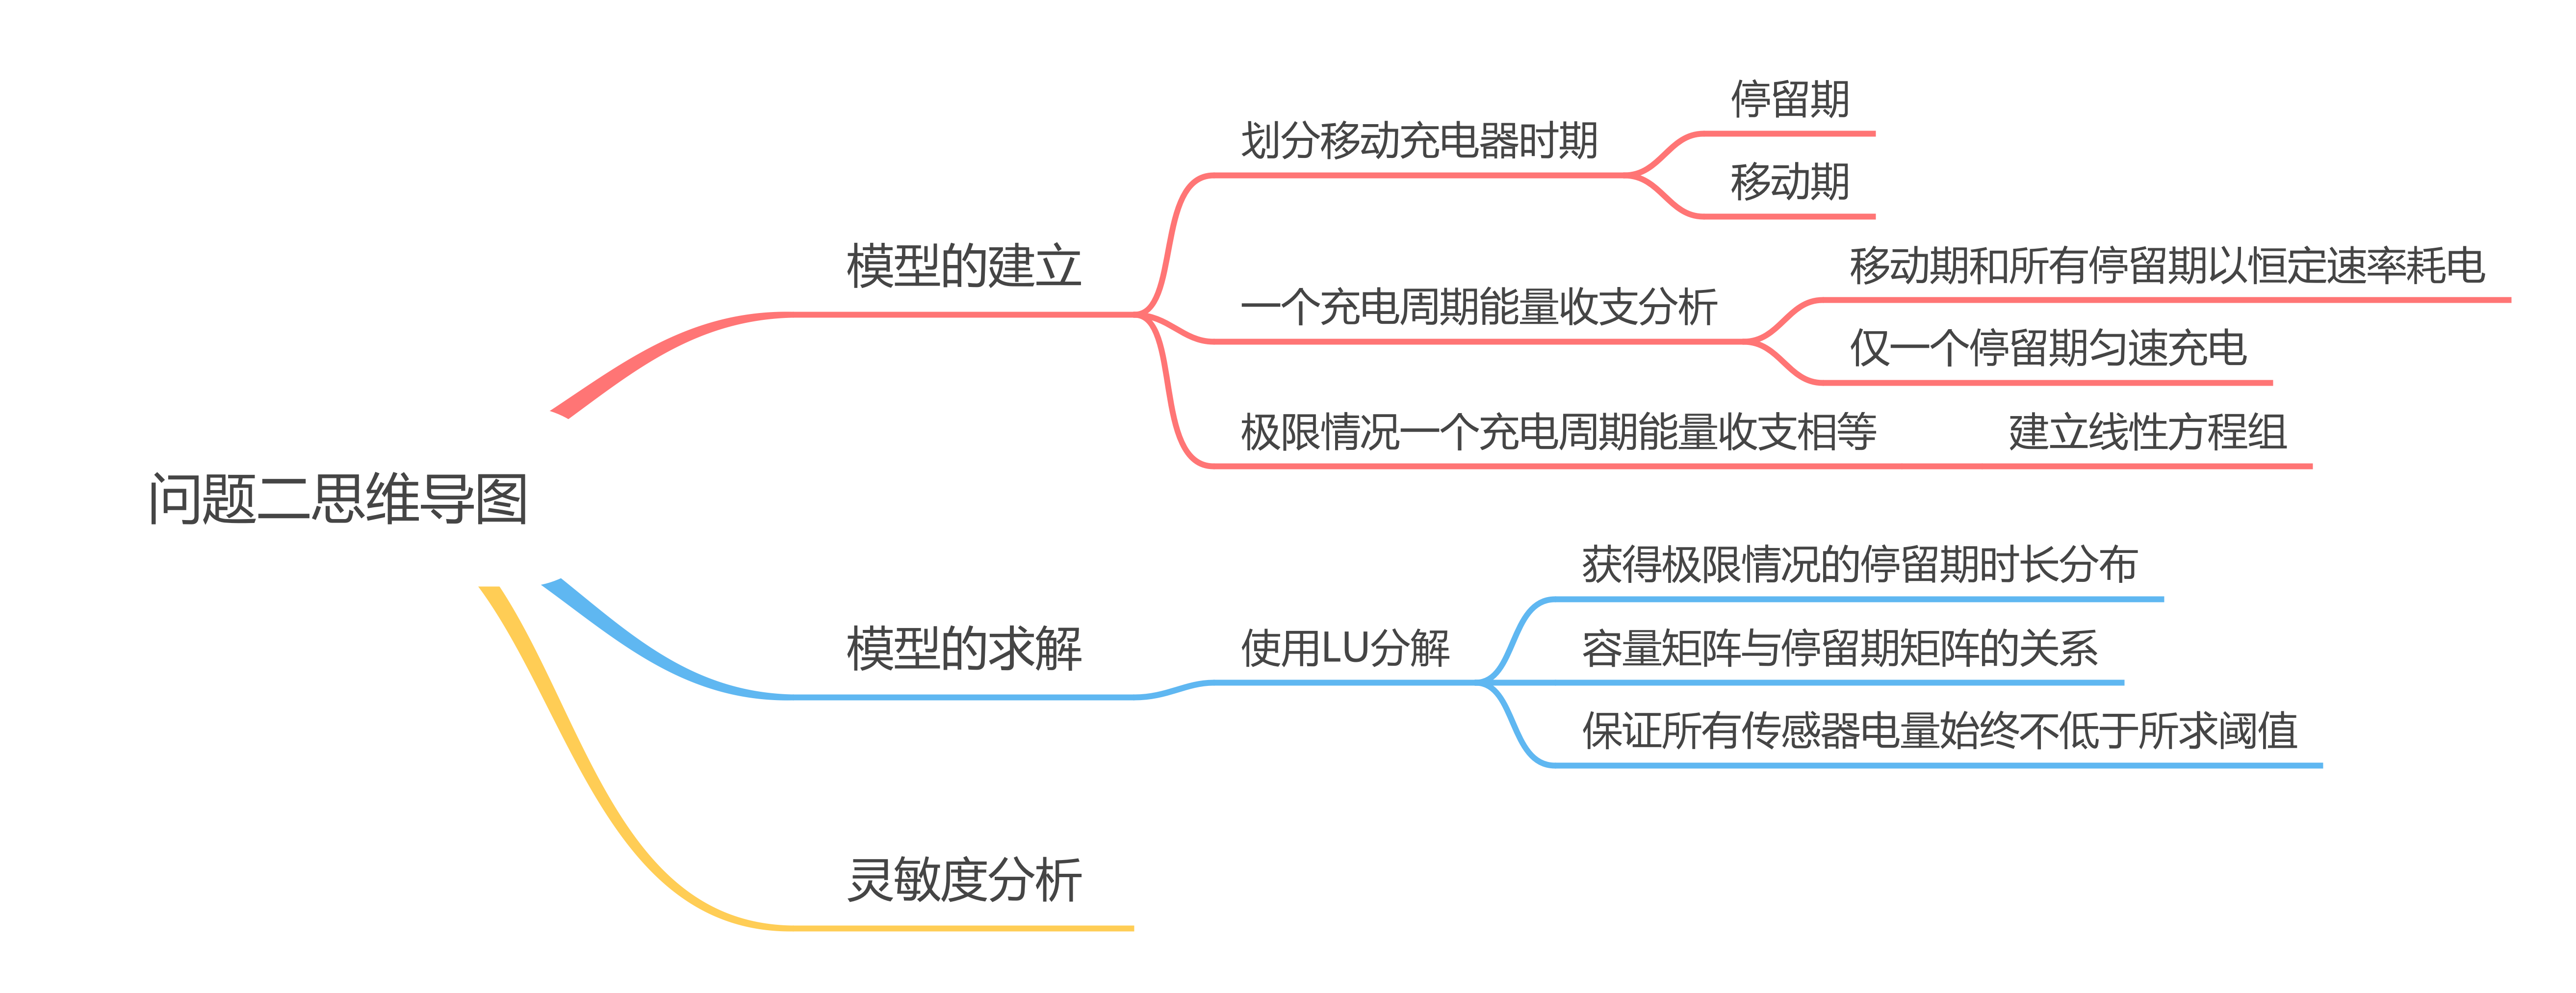
\includegraphics[width=\textwidth]{figures/222222.png}
                \caption{问题二思维流程图}\label{ssssct}
            \end{figure}

        \subsection{模型的建立}
            在周期$T$的模型中,MC循环遍历路径,在预定区域充电。周期$T$分为驻留期$T_{park}$和移动期$T_{traverse}$。驻留期MC静止于传感器充电范围,匀速充电;移动期MC匀速移动,停止供电。能量流动表达式为:
            \begin{gather}\label{ssssssss}
                c_j \cdot (T_{traverse} + \sum_{i} T_{park}^i) \leq r \cdot T_{park}^j, \quad j=1,2,\dots,n,
            \end{gather}
            其中左端和右端分别表示耗能和供能。极限情况下,传感器获得能量等于消耗能量,得到$n$元线性方程组:
            \begin{gather}
                c_j \cdot (L/v + \sum_{i=1}^{n} t_i) = r \cdot t_j, \quad j=1,2,\dots,n,
            \end{gather}
            其中$n$为传感器数,$L$为问题一总里程,$v$为MC速度,$c_j$为第$j$个传感器耗电速率,$r$为充电速率。求解得到驻留时间$t_i$。

            传感器电量需始终大于阈值$f$,电池容量$T_{threshold}$不低于驻留期补充能量:
            \begin{gather}
                \left\{
                \begin{matrix}
                    v_1 \geq f + r \cdot t_1 \\
                    v_2 \geq f + r \cdot t_2 \\
                    \vdots \\
                    v_n \geq f + r \cdot t_n
                \end{matrix}
                \right.,
            \end{gather}
            极限情况下:
            \begin{gather}
                \bm{V_{threshold}} = \bm{F} + r \cdot \bm{T_{threshold}},
            \end{gather}
            其中$\bm{F}$为全$f$的$n \times 1$向量,$\bm{T_{threshold}}$为$t_1, t_2, \dots, t_n$的$n \times 1$向量。

        \subsection{模型的求解}
            使用$LU$分解求解线性方程组,计算复杂度为$O(n^3)$,无需判定矩阵正定,浮点操作量为$O(n^2)$。化简为矩阵方程:
            \begin{gather}
                \bm{A} \cdot \bm{T_{threshold}} = -\frac{L}{v} \cdot \bm{b},
            \end{gather}
            或:
            \begin{gather}
                \begin{bmatrix}
                    1 - \frac{r}{c_1} & 1 & \dots & 1 \\
                    1 & 1 - \frac{r}{c_2} & \dots & 1 \\
                    \vdots & \vdots & \ddots & \vdots \\
                    1 & 1 & \dots & 1 - \frac{r}{c_n}
                \end{bmatrix}
                \begin{bmatrix}
                    t_1 \\ t_2 \\ \vdots \\ t_n
                \end{bmatrix}
                = -\frac{L}{v}
                \begin{bmatrix}
                    1/c_1 \\ 1/c_2 \\ \vdots \\ 1/c_n
                \end{bmatrix}.
            \end{gather}
            $LU$分解:
            \begin{gather}
                \bm{Ly} = -\frac{L}{v} \cdot \bm{b}, \quad
                \left\{
                \begin{matrix}
                    y_1 = b_1 \\
                    y_k = b_k - \sum_{j=1}^{k-1} l_{kj} y_j
                \end{matrix}
                \right., \quad k=2,3,\dots,n, \\
                \bm{U T_{threshold}} = \bm{y}, \quad
                \left\{
                \begin{matrix}
                    t_n = y_n / u_{nn} \\
                    t_k = (y_k - \sum_{j=k+1}^{n} u_{kj} t_j) / u_{kk}
                \end{matrix}
                \right., \quad k=n-1,\dots,1.
            \end{gather}
            结果如表~\ref{biao2}所示:

            \begin{table}[H]
                \setstretch{1.4}
                \centering
                \caption{传感器电池最小容量分布}\label{biao2}
                \begin{tabular}{cccc}
                    \toprule[2pt]
                    \multicolumn{1}{m{2.5cm}}{\centering 传感器序号} &
                    \multicolumn{1}{m{4.5cm}}{\centering 传感器最小电池容量} &
                    \multicolumn{1}{m{2.5cm}}{\centering 传感器序号} &
                    \multicolumn{1}{m{4.5cm}}{\centering 传感器最小电池容量} \\
                    \midrule[1pt]
                    2 & 5001.24202643 & 3 & 4801.81519446 \\
                    1 & 5533.04691166 & 4 & 5023.40056331 \\
                    9 & 4801.81519446 & 22 & 5466.57130101 \\
                    7 & 5023.40056331 & 28 & 5023.40056331 \\
                    6 & 4602.38836250 & 24 & 4801.81519446 \\
                    14 & 4801.81519446 & 23 & 4580.22982561 \\
                    11 & 5222.82739527 & 21 & 5023.40056331 \\
                    8 & 4823.97373135 & 29 & 5466.57130101 \\
                    12 & 4801.81519446 & 26 & 4580.22982561 \\
                    15 & 5023.40056331 & 25 & 5023.40056331 \\
                    27 & 4801.81519446 & 18 & 4757.49812069 \\
                    16 & 5444.41276412 & 19 & 4602.38836250 \\
                    13 & 5244.98593216 & 20 & 5222.82739527 \\
                    10 & 4801.81519446 & 17 & 5001.24202643 \\
                    5 & 4646.70543627 & & \\
                    \bottomrule[2pt]
                \end{tabular}
            \end{table}

        \subsection{灵敏度分析}
            改变MC移动速度$v$、充电速率$r$、充电半径$R$和电量阈值$f$,观察电池容量变化,如图~\ref{mgh}所示:

            \begin{figure}[H]
                \centering
                \subfigure[移动速度$v$影响]{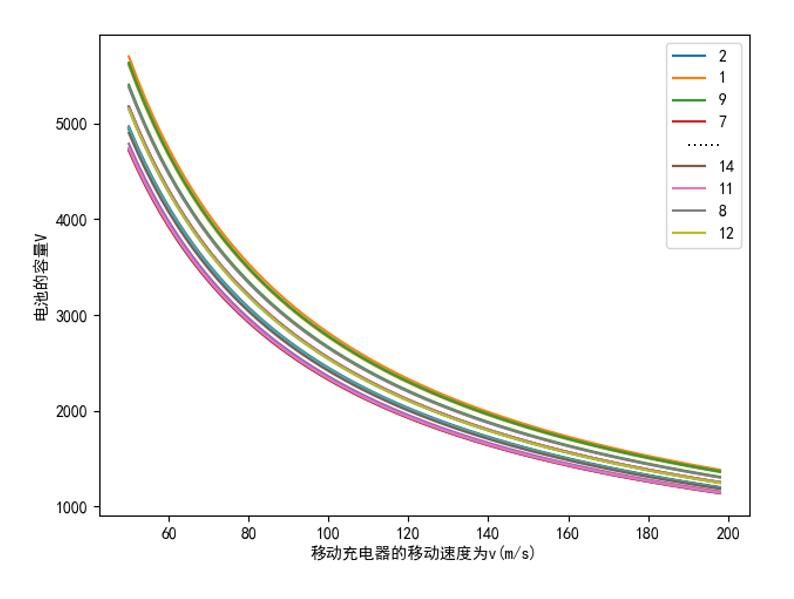
\includegraphics[height=6.5cm,width=7.5cm]{2333v.jpg}}
                \subfigure[充电速率$r$影响]{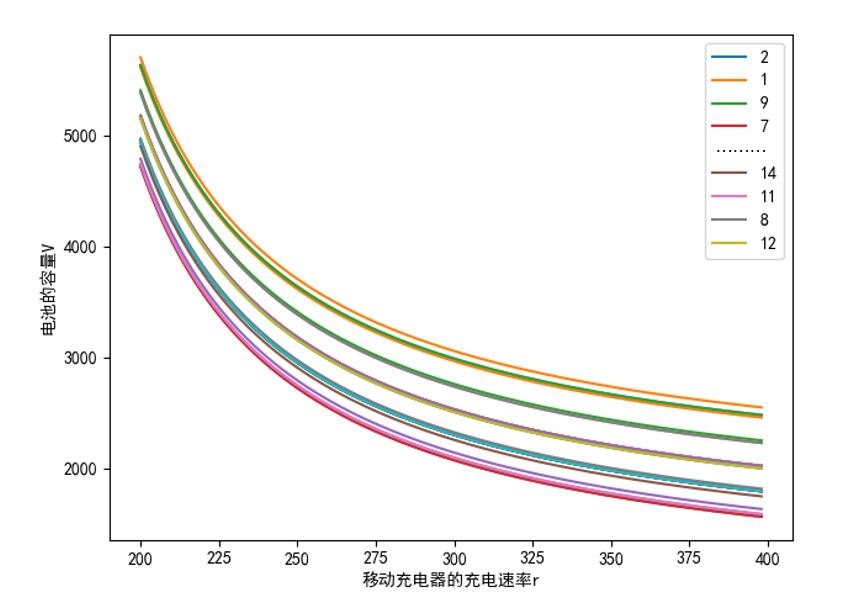
\includegraphics[height=6.5cm,width=7.5cm]{2333r.jpg}}
            \end{figure}
            \begin{figure}[H]
                \centering
                \subfigure[充电半径$R$影响]{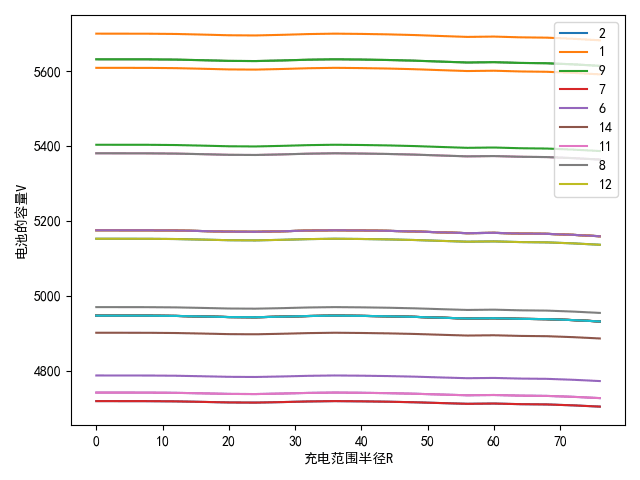
\includegraphics[height=6.5cm,width=7.5cm]{2333R.png}}
                \subfigure[电量阈值$f$影响]{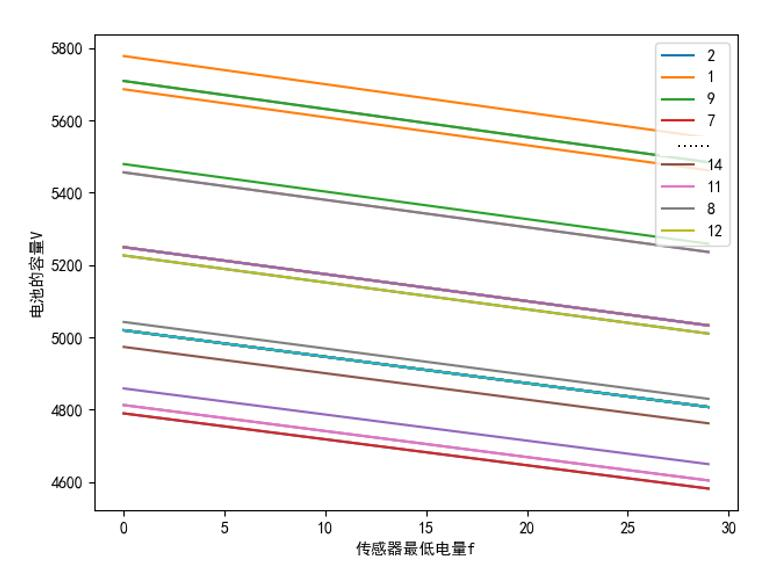
\includegraphics[height=6.5cm,width=7.5cm]{2333f.jpg}}
                \caption{不同参数对电池容量的影响}\label{mgh}
            \end{figure}

            图~\ref{mgh}(c)显示,当$R$在$0$到$70m$变化时,电池容量变化小,表明$R$对容量需求影响有限。图~\ref{mgh}(a)、(b)、(d)显示$v$、$r$、$f$与容量负相关。$f$增大时容量线性降低,因$r$远大于$c_j$,使驻留时间$t_i$减少效应大于$f$增大效应,符合实际。

    % Problem 3: Model establishment and solution
    \section{问题三模型的建立与求解}
        \subsection{问题描述与分析}
            问题三要求设计4辆MC的充电路线,最小化总能量消耗。为避免重复充电,每个传感器仅由一辆MC充电。当$R=0$,问题为多旅行商问题(MTSP)。在问题一基础上,设计插板式编码嵌入LGA,以总路程为目标优化。思维流程图如图~\ref{asdf3}所示:

            \begin{figure}[H]
                \centering
                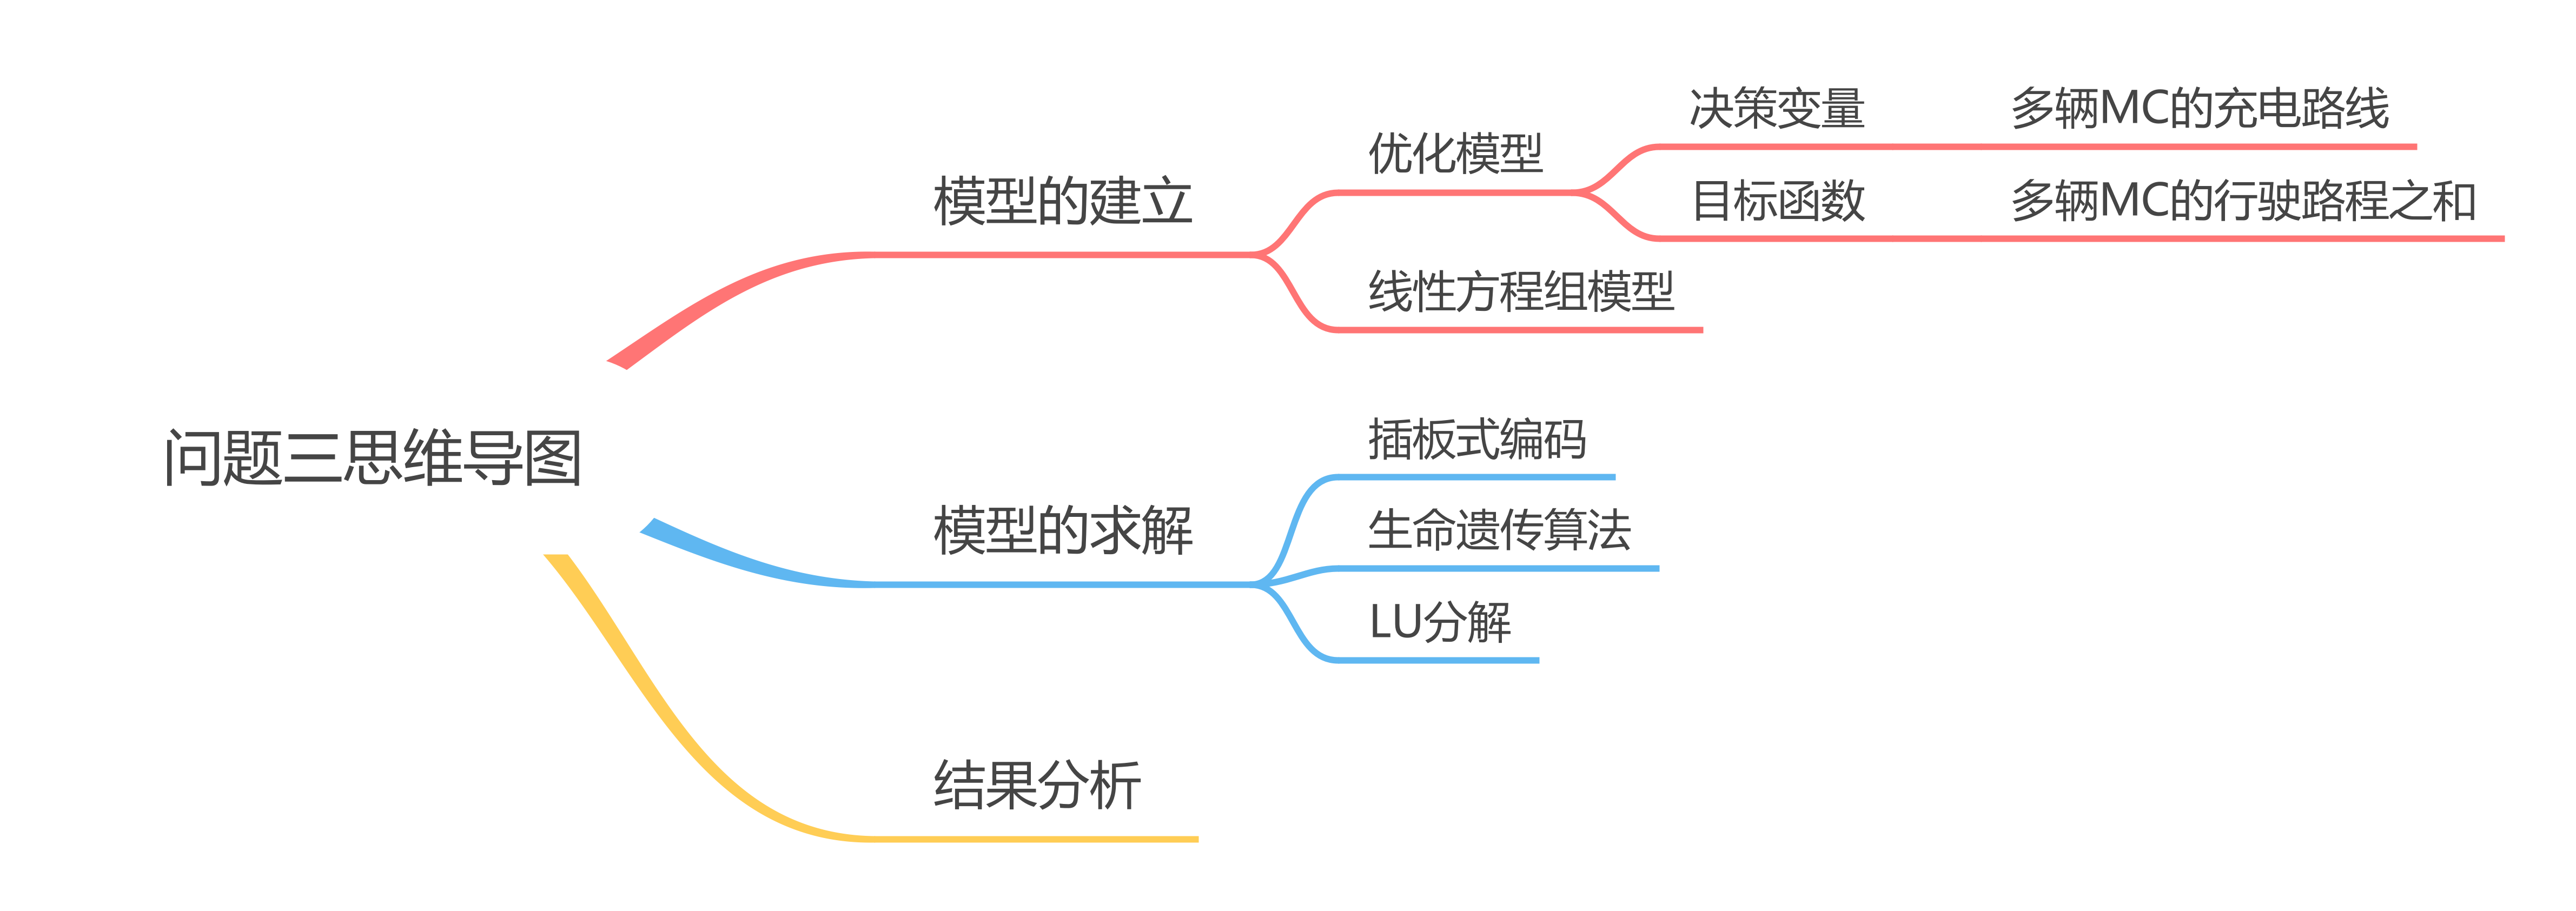
\includegraphics[width=\textwidth]{figures/3.png}
                \caption{问题三思维流程图}\label{asdf3}
            \end{figure}

        \subsection{多TSP模型建立}
            4辆MC的总决策序列为:
            \begin{gather*}
                P_n = \{[p_1, \dots, p_i]_1, [p_{i+1}, \dots, p_j]_2, [p_{j+1}, \dots, p_k]_3, [p_{k+1}, \dots, p_{29}]_4\},
            \end{gather*}
            每辆MC路径为:
            \begin{gather*}
                B_k = [p_i, p_{i+1}, \dots, p_j]_k,
            \end{gather*}
            总路径:
            \begin{gather*}
                P_n = \{B_1, B_2, B_3, B_4\}.
            \end{gather*}
            路径$B_k$的路程为:
            \begin{gather*}
                L(B_k) = d(p_0, p_i) + d(p_0, p_j) + \sum_{r=i}^{j-1} d(p_r, p_{r+1}),
            \end{gather*}
            目标函数为:
            \begin{gather}
                L(P_n) = \sum_{i=1}^{4} L(B_i),
            \end{gather}
            优化模型为:
            \begin{gather}
                \min L(P_n), \\
                s.t. \left\{
                \begin{matrix}
                    p_i(x_i, y_i) \in S, (1 \leqslant i \leqslant 29, i \in \mathbb{Z}), \\
                    \forall i \neq j, p_i \neq p_j.
                \end{matrix}
                \right.
            \end{gather}

        \subsection{插板式编码}
            为表示多辆MC路径,在染色体中插入无意义挡板基因。例如,两辆MC时:
            \begin{gather*}
                P_n = \{[p_1, \dots, p_i]_1, [p_{i+1}, \dots, p_{29}]_2\},
            \end{gather*}
            染色体为:
            \begin{gather*}
                A_n = [a_{n1}, \dots, a_{ni}, \varphi, a_{ni+1}, \dots, a_{n29}],
            \end{gather*}
            其中$\varphi$为挡板基因。4辆MC插入3个挡板,分成4段。挡板基因参与交叉和变异。引入冗余惩罚因子:
            \begin{gather}
                \theta(P_n) = \left\{
                \begin{matrix}
                    1, & \exists (Loc(\varphi_i) + 1 = Loc(\varphi_{i+1})) \vee \exists (Loc(\varphi_i) = 0) \vee \exists (Loc(\varphi_i) = \text{size}(A_n)), \\
                    0, & \text{otherwise},
                \end{matrix}
                \right.
            \end{gather}
            其中$Loc(\varphi_i)$为挡板位置,$size(A_n)$为染色体维数。目标函数为:
            \begin{gather}
                F(P_n) = L(P_n) + \theta(P_n) M,
            \end{gather}
            其中$M$为大正系数。

        \subsection{结果分析}
            设置参数$r=200mA/s$,$f=10mA$,$v=50m/s$,结果如图~\ref{gdfsdf}所示:

            \begin{figure}[H]
                \centering
                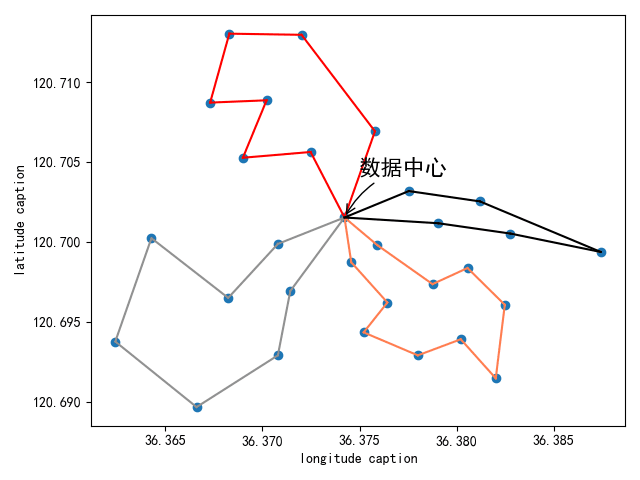
\includegraphics[width=.8\textwidth]{figures/s3.png}
                \caption{四辆移动充电装置路径图}\label{gdfsdf}
            \end{figure}

            4辆MC的路线和耗时如表~\ref{bidsao2}所示:

            \begin{table}[H]
                \setstretch{1}
                \centering
                \caption{每个传感器的移动路径}\label{bidsao2}
                \begin{tabular}{ccc}
                    \toprule[2pt]
                    \multicolumn{1}{m{2.5cm}}{\centering 传感器序号} &
                    \multicolumn{1}{m{4.5cm}}{\centering 移动路径} &
                    \multicolumn{1}{m{2.5cm}}{\centering 耗时} \\
                    \midrule[1pt]
                    1 & [0, 1, 9, 7, 6, 11, 14, 15, 12, 8, 2, 0] & 59 \\
                    2 & [0, 4, 21, 22, 23, 24, 28, 3, 0] & 66 \\
                    3 & [0, 17, 19, 29, 26, 25, 18, 20, 0] & 77 \\
                    4 & [0, 10, 16, 27, 13, 5, 0] & 57 \\
                    \bottomrule[2pt]
                \end{tabular}
            \end{table}

            电池容量分布如表~\ref{adfs}所示:

            \begin{table}[H]
                \setstretch{0.7}
                \centering
                \caption{传感器电池最小容量分布}\label{adfs}
                \begin{tabular}{cccc}
                    \toprule[2pt]
                    \multicolumn{1}{m{2.5cm}}{\centering 传感器序号} &
                    \multicolumn{1}{m{4.5cm}}{\centering 传感器最小电池容量} &
                    \multicolumn{1}{m{2.5cm}}{\centering 传感器序号} &
                    \multicolumn{1}{m{4.5cm}}{\centering 传感器最小电池容量} \\
                    \midrule[1pt]
                    1 & 415.765 & 28 & 369.935 \\
                    9 & 556.166 & 3 & 494.6706 \\
                    7 & 363.116 & 17 & 502.970 \\
                    6 & 421.616 & 19 & 686.930 \\
                    11 & 310.466 & 29 & 433.985 \\
                    14 & 363.116 & 26 & 510.635 \\
                    15 & 474.266 & 25 & 365.00 \\
                    12 & 368.9666 & 18 & 433.9851 \\
                    8 & 363.116 & 20 & 579.6201 \\
                    2 & 421.616 & 10 & 345.184 \\
                    4 & 429.020 & 16 & 481.3847 \\
                    21 & 586.580 & 27 & 294.109 \\
                    22 & 369.935 & 13 & 350.859 \\
                    23 & 435.585 & 5 & 243.0347 \\
                    24 & 310.850 & & \\
                    \bottomrule[2pt]
                \end{tabular}
            \end{table}

            对比问题一、二,4辆MC的总能量消耗高于单MC,但传感器最小电池容量平均值降低,表明增派MC可降低电池容量需求。

    % Model evaluation
    \section{模型的评价}
        \subsection{模型的优点}
            \begin{itemize}
                \item[(1)] 结合无线能量传输技术,在固定周期遍历充电模型基础上引入充电半径,建立单MC和多MC能耗模型,拓宽应用范围。
                \item[(2)] 从时间维度考察能量收支,利用$LU$分解求解电池容量分布,计算复杂度低,无需判定矩阵正定。
                \item[(3)] 设计生命遗传算法,结合插板编码,防止陷入局部最优,兼顾局部和全局搜索能力。
            \end{itemize}

        \subsection{模型的缺点}
            LGA嵌入SGD时搜索时间较长,时间复杂度需改进。

    % References
    \newpage
    \addcontentsline{toc}{section}{参考文献}
    \nocite{*}
    \begin{thebibliography}{9}
        \bibitem{1} Othman M F, Shazali K. Wireless sensor network applications: A study in environment monitoring system[J]. Procedia Engineering, 2015, 41: 1204-1210.
        \bibitem{2} Borges L M, Velez F J, Lebres A S. Survey on the characterization and classification of wireless sensor network applications[J]. IEEE Communications Surveys \& Tutorials, 2014, 16(4): 1860-1890.
        \bibitem{3} Xie L, Shi Y, Hou Y T, et al. Making sensor networks immortal: An energy-renewal approach with wireless power transfer[J]. IEEE/ACM Transactions on Networking, 2012, 20(6): 1748-1761.
        \bibitem{4} Tarng W, Ou K L, Huang K J, et al. Applying cluster merging and dynamic routing mechanisms to extend the lifetime of wireless sensor networks[J]. International Journal of Communication Networks and Information Security, 2011, 3(1): 8.
        \bibitem{5} 曲立军, 党鑫, 武继刚. 无线传感器网络中的充电调度算法[J]. 计算机与数字工程, 2017, 45(2): 319-326.
        \bibitem{6} Butler Z, Rus D. Controlling mobile sensors for monitoring events with coverage constraints[C]//IEEE International Conference on Robotics and Automation, 2004. Proceedings. ICRA'04. 2004. IEEE, 2004, 2: 1568-1573.
        \bibitem{7} Yao W, Li M, Wu M Y. Inductive charging with multiple charger nodes in wireless sensor networks[C]//Asia-Pacific Web Conference. Springer, Berlin, Heidelberg, 2006: 262-270.
    \end{thebibliography}

\end{document}